\documentclass[11pt]{article}
%\usepackage{abbrevs}
\usepackage{natbib}
\usepackage{hyperref}
\usepackage{float}
\usepackage[pdftex]{graphicx}     % could insert ``draft'' between []
\usepackage{stmaryrd}
\usepackage{appendix}
\pagestyle{empty}

\setlength{\oddsidemargin}{0pt} % there is 1 inch before the
                                % side margin in ``article'' class
\setlength{\textwidth}{6.5in}

\setlength{\voffset}{0pt}
\setlength{\topmargin}{-0.75in}     % there is 1 inch before the
                                % top margin in ``article'' class and
                                % then room for header, etc.
\setlength{\textheight}{10.0in}
%%%%%%%%%%%

\newcommand{\inch}{$^{\prime\prime}$}
\newcommand{\foot}{$^{\prime}$}
\renewcommand{\deg}{^\circ}

\begin{document}
\title{HERA Installation Procedure}
\author{David DeBoer}
\maketitle

\setcounter{tocdepth}{3}
\tableofcontents

\section{Pole Installation}
After surveying the entire plat, the poles are installed on center with a $\pm$10cm tolerance, per Figure \ref{fig:poles}.  The number of rows and poles per row is set by the hex order.  Table \ref{tab:hexnums} shows important numbers for different orders.
\begin{figure}[H]
\centering
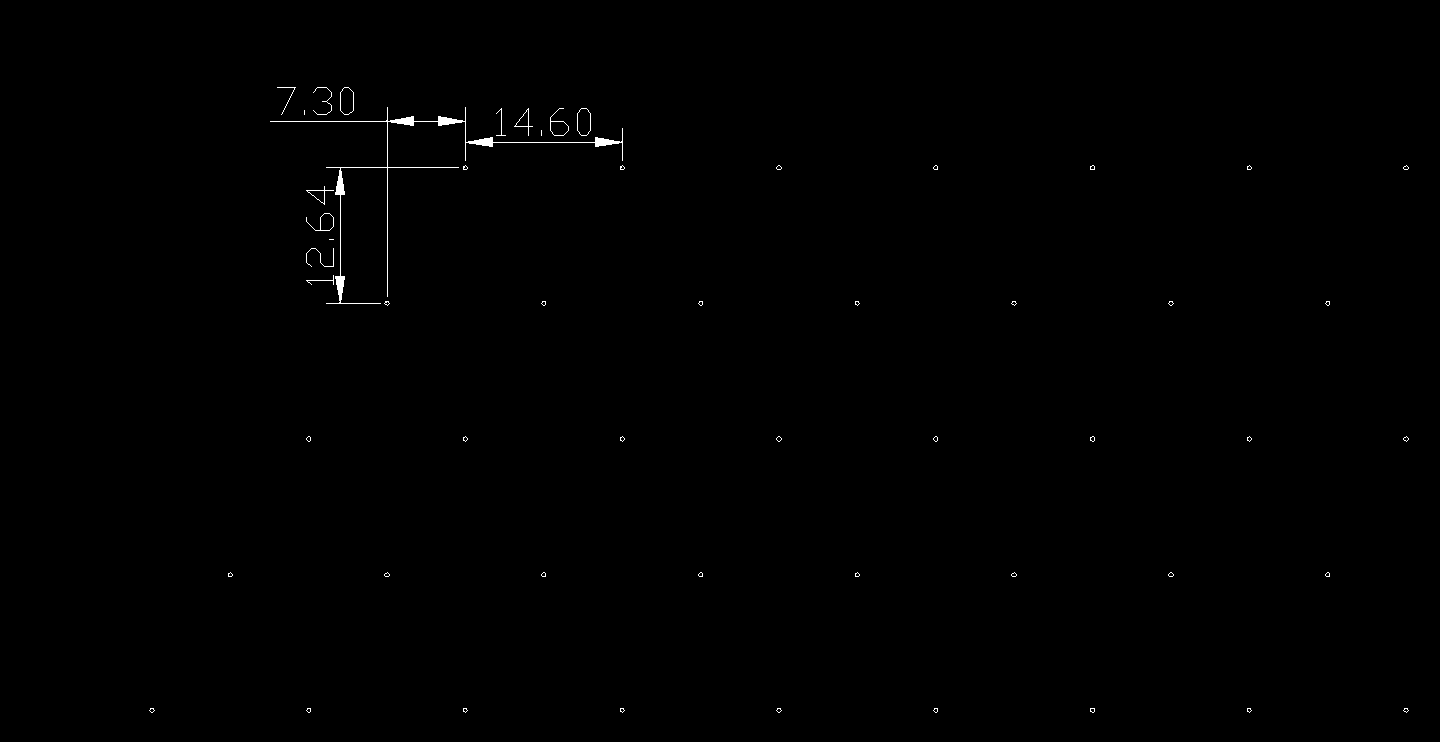
\includegraphics[width=\textwidth]{graphics/bigPoles.png}
\label{fig:poles}
\caption{Layout of poles.  Dimensions in meters.}
\end{figure}

\begin{table}[H]
\centering
\caption{Numbers}.
\begin{tabular}{| l | l |} \hline
order & total number \\ \hline
4 & x \\ \hline
\end{tabular}
\label{tab:hexnums}
\end{table}

\section{Pole Height}
Each trio of poles supports an antenna and each interior pole is shared by three antennas.  A fiducial constant height must be measured for each trio and marked with a small eye-bolt.  From within the circle circumscribed by the poles, this height may be measured by a theodolite along a bubble-level line or by a total station at constant $z$.  This height should be about 1.5-meters above the ground.
\begin{figure}[H]
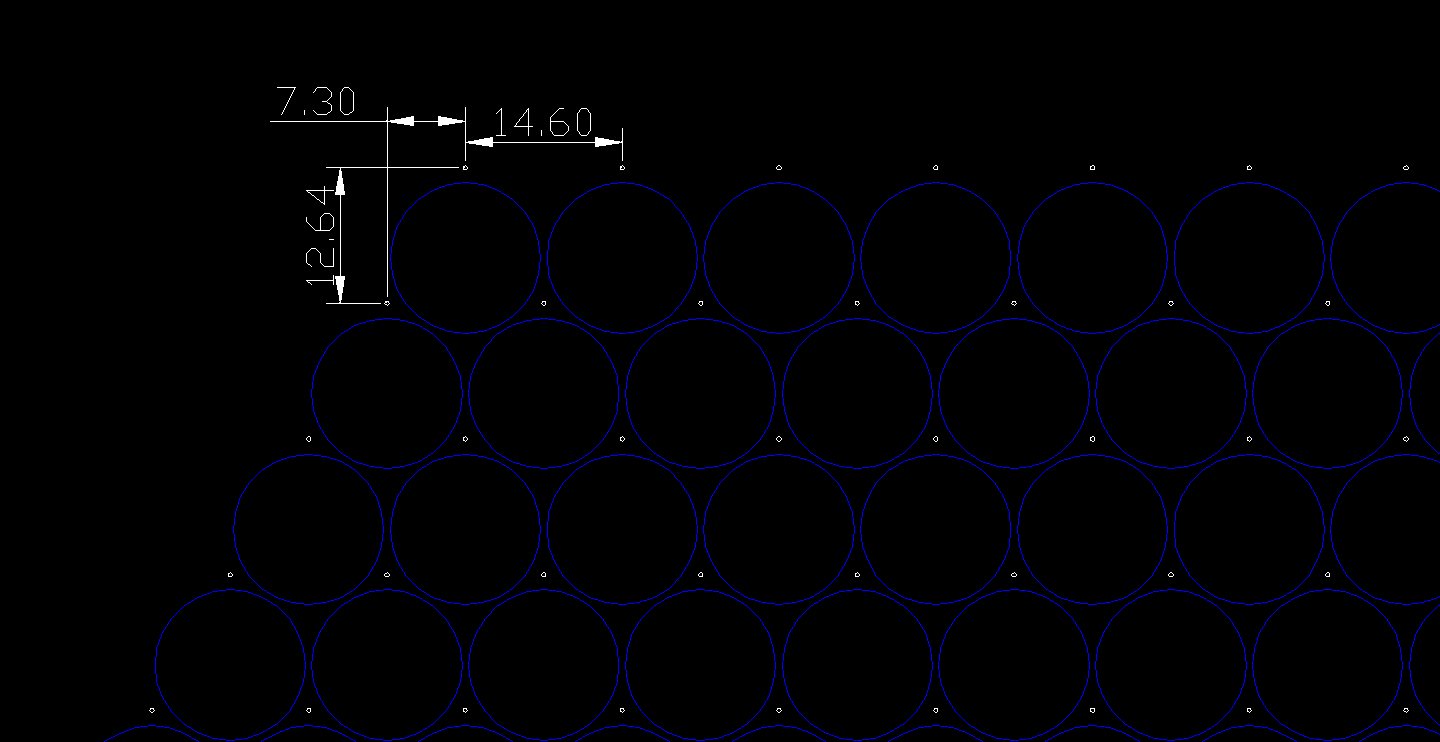
\includegraphics[width=\textwidth]{graphics/poles_and_ants.png}
\label{fig:poles_ants}
\caption{Layout of poles.  Dimensions in meters.}
\end{figure}

\section{Hub Centering and Leveling}
With each pole with a constant height eye-bolt, the following is used to center the hub center:
\subsection{Radial lines}
A arrangement of three fixed length lines and three match spring attached on a small inner ring with a plumb-bob is used. See Figure refPicture.

\subsection{Jig}
With the center point defined by the radial lines and hanging bob, a jig as described below is used.

\newpage
\appendix
\section{Checklist}

\renewcommand{\labelitemi}{$\boxempty$}
\renewcommand{\labelitemii}{$\boxempty$}
\begin{itemize}
\item Install poles
\item Survey pole marker fiducial heights ($\approx$ 1.5m) and install eye-bolts
\item Install centering jig (H7jcen)
\item Install hub forms with hub jig (H7jhub), using H7jcen to center
\item Rotate hub to point to poles and conduit exit to correct direction
\item Level with H7jhub and stakes
\item Install hub sleeves (top, bottom and exit) and rebar
\item Pour concrete and let set
\item Mark center point on rebar with cable tie (this is the vertex) and remove jigs
\item Set-up Total Station on center and 60in above rebar
\item Survey and install pole vertical assemblies (H1p2v)
	\begin{itemize}
	\item bottom at z=14.33in
	\item shim so vertical
	\item use qty 3 3/8'' lag bolts
	\end{itemize}
\item Survey and install pole horizontal assembly (H1p2h):  target at angle = 8.233$^\circ$, distance = 272.11in (z = 39in)
\item Rough in posts (H1pxxx) between the poles using rim pieces (H1vvvvv), including post forms (   )
\item If unshared post or first installation of a shared post, survey and brace:  target at angle = 8.233$^\circ$, distance = 272.11in (z=39in)
\item If shared post, survey using the offset piece (H1ggggg) and brace:  target at ...
\item Install rebar and concrete,  let set and remove bracing
\item Install horizontal pvc support pieces in hub, level and affix
\item Install parabolic spars in hub (be sure pre-drilled holes are facing up) and affix at ends
\item Install pvc cross pieces ( )
\item Install cross piece spars and affix at ends
\item Install hub access platform at appropriate location
\item Install all wire cloth panel A pieces
\item Install all but access section of panel B pieces (with furring strips on outer), sandwiching A-B-cross
\item Install all but access section of panel C pieces (with furring strips on outer), sandwiching B-C-furring
\item Install all panel D pieces, sandwiching C-D-furring
\item Install all panel E pieces
\item install door pieces
\end{itemize}

\bibliographystyle{plainnat}
\bibliography{YOUR BIBLIOGRAPHY HERE}
\end{document}
